\section{Trigger di Schmitt}

\begin{figure}[h]
	\centering
	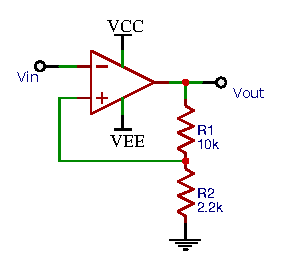
\includegraphics[scale=1]{circ_schmidt.pdf}
	\caption{trigger di Schmitt}
	\label{f:trigger}
\end{figure}

Si è montato il circuito in \fig{trigger} e si sono misurati con il multimetro le resistenze $R_1= \SI{9.93(9)}{\kohm}$ e $R_2=\SI{2.27(3)}{\kohm}$. Il trigger di Schmitt è un comparatore di soglia con isteresi: ha dunque due valori di soglia in ingresso che sono $V_{T}= V_{O}\frac{R_2}{R_1+R_2}$ al variare dei due valori possibile per $V_O$.
\begin{figure}[h]
	\centering
	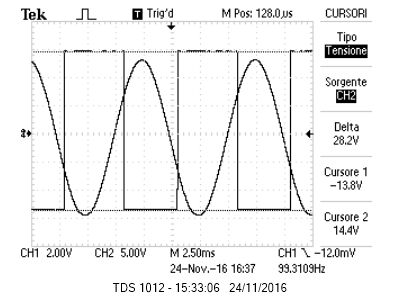
\includegraphics[scale=0.7]{parteC_sinusoide.png}
	\caption{Risposta del trigger ad un ingresso sinusoidale.}
	\label{f:sinusoide}
\end{figure}
In \fig{sinusoide} si mostra la risposta del trigger ad un ingresso sinusoidale con frequenza e ampiezza tale da permettere un corretto funzionamneto del circuito.
Quando l'ingresso $V_{in}$ è minore della soglia bassa $V_{TL}$ allora l'uscita assume il valore basso $V_{OL} \approx V_{EE}$. Mentre $V_{in}$ è compreso tra le due soglie l'uscita viene mantenuta al valore assunto prima di varcare la soglia bassa. Quando $V_{in}$ supera la soglia alta $V_{TH}$ l'uscita si porta ad un valore $V_{OH} \approx V_{CC}$. 
Se invece l'ingresso è all'inizio maggiore di $V_{TH}$ e poi se ne inizia a diminuire l'ampiezza, allora il trigger scatta quando $V_{in}$ diventa minore di $V_{TL}$ e l'uscita si regola sul valore basso $V_{OL}$.

\begin{figure}[h]
	\centering
	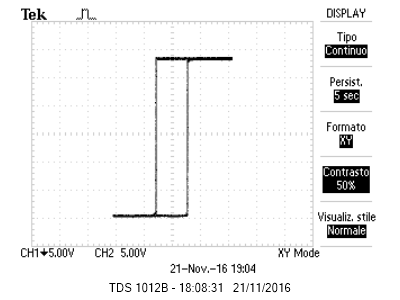
\includegraphics[scale=1]{partec_isteresi.png}
	\caption{uscita in funzione dell'ingresso.}
	\label{f:isteresi}
\end{figure}
Tale funzionamento realizza un' isteresi tra ingresso e uscita come è visibile nella \fig{isteresi}.

Una caratteristica importante di tale trigger che lo differenzia dai comparatori con una sola soglia è il fatto che,in presenza di un segnale di rumore che oscilla intorno ad una soglia l'uscita non oscilla a sua volta perchè il trigger scatta al massimo una volta.
Si sono misurati con l'oscilloscopio $V_{OL}= \SI{-14.0(1)}{\V}$ e  $V_{OH}= \SI{14.5(1)}{\V}$ e le due soglie dell'ingresso e si sono confrontate le misure con i valori attesi ricavati dalla formula prima scritta.
\begin{table}[h]
	\centering
	\begin{tabular}{ *{2}{S[table-figures-exponent = 2]} }
		{$V_{T,atteso}$ [\SI{}{\V}]} & {$V_{T,misurato}$ [\SI{}{\V}]} \\
		\midrule
		 $\SI{2.66(5)}{}$	&	$\SI{2.72(2)}{}$	\\
		$\SI{-2.69 (5)}{}$	&	$\SI{-2.64 (2)}{}$	\\
	\end{tabular}
	\caption{Tensioni di soglia del trigger misuarate e attese.}
	\label{t:trigg_soglia}
\end{table}
Si nota dalla tabella che i valori attesi e misurati sono tra di loro compatibili.

Diminuendo l'ampiezza del segnale in ingresso si è ottenuto il grafico in \fig{sotto_soglia}.
\begin{figure}[h]
	\centering
	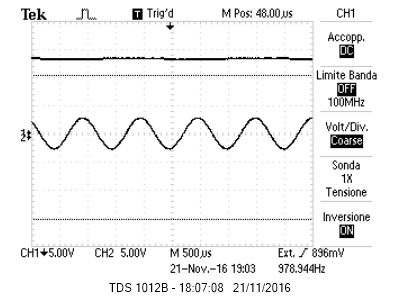
\includegraphics[scale=1]{partec_ampiezza_bassa.png}
	\caption{Ampiezza di $V_{in}$ sotto soglia. }
	\label{f:sotto_soglia}
\end{figure}

Si nota che il massimo di $V_{in}$ fa scattare il trigger, che regola quindi l'uscita a $V_{OH}$. Essendo il segnale non simmetrico, il minimo di $V_{in}$ non è minore della soglia negativa $V_{TL}$ quindi il trigger non scatta e l'uscita resta quindi impostata sul livello alto.

\begin{figure}[h]
	\centering
	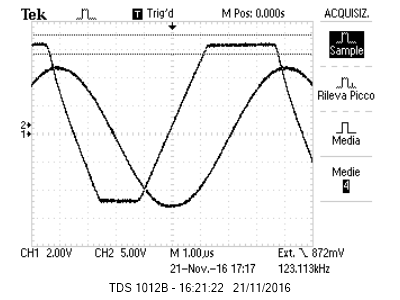
\includegraphics[scale=1]{slew_rateC.png}
	\caption{Evidenza dello slew rate dell'OpAmp per frequeze dell'ordine di $\SI{100}{\kHz}$}
	\label{f:slew_rate}
\end{figure}

All'aumentare della frequenza del segnale in ingresso si possono avere degli effetti dovuti allo slew rate dell'OpAmp come in \fig{slew_rate}.Infatti il tempo di commutazione del segnale in uscita tra livello alto e basso non è istantanea e tale aspetto è messo in evidenza proprio ad alte frequenze. Infatti in tale regime l'OpAmp impiegando un certo tempo per commutare l'uscita , questa non è più un onda quadra ma bensì presenta dei fronti di discesa e salita con una pendenza in modulo pari a $\SI{12.7}{\volt\per\micro\s}$.
